\documentclass{ximera}
\graphicspath{  %% When looking for images,
{./}            %% look here first,
{./pictures/}   %% then look for a pictures folder,
{../pictures/}  %% which may be a directory up.
{../../pictures/}  %% which may be a directory up.
{../../../pictures/}  %% which may be a directory up.
{../../../../pictures/}  %% which may be a directory up.
}

\usepackage{listings}
%\usepackage{circuitikz}
\usepackage{xcolor}
\usepackage{amsmath,amsthm}
\usepackage{subcaption}
\usepackage{graphicx}
\usepackage{tikz}
%\usepackage{tikz-3dplot}
\usepackage{amsfonts}
%\usepackage{mdframed} % For framing content
%\usepackage{tikz-cd}

  \renewcommand{\vector}[1]{\left\langle #1\right\rangle}
  \newcommand{\arrowvec}[1]{{\overset{\rightharpoonup}{#1}}}
  \newcommand{\ro}{\texttt{R}}%% row operation
  \newcommand{\dotp}{\bullet}%% dot product
  \renewcommand{\l}{\ell}
  \let\defaultAnswerFormat\answerFormatBoxed
  \usetikzlibrary{calc,bending}
  \tikzset{>=stealth}
  




%make a maroon color
\definecolor{maroon}{RGB}{128,0,0}
%make a dark blue color
\definecolor{darkblue}{RGB}{0,0,139}
%define the color fourier0 to be the maroon color
\definecolor{fourier0}{RGB}{128,0,0}
%define the color fourier1 to be the dark blue color
\definecolor{fourier1}{RGB}{0,0,139}
%define the color fourier 1t to be the light blue color
\definecolor{fourier1t}{RGB}{173,216,230}
%define the color fourier2 to be the dark green color
\definecolor{fourier2}{RGB}{0,100,0}
%define teh color fourier2t to be the light green color
\definecolor{fourier2t}{RGB}{144,238,144}
%define the color fourier3 to be the dark purple color
\definecolor{fourier3}{RGB}{128,0,128}
%define the color fourier3t to be the light purple color
\definecolor{fourier3t}{RGB}{221,160,221}
%define the color fourier0t to be the red color
\definecolor{fourier0t}{RGB}{255,0,0}
%define the color fourier4 to be the orange color
\definecolor{fourier4}{RGB}{255,165,0}
%define the color fourier4t to be the darker orange color
\definecolor{fourier4t}{RGB}{255,215,0}
%define the color fourier5 to be the yellow color
\definecolor{fourier5}{RGB}{255,255,0}
%define the color fourier5t to be the darker yellow color
\definecolor{fourier5t}{RGB}{255,255,100}
%define the color fourier6 to be the green color
\definecolor{fourier6}{RGB}{0,128,0}
%define the color fourier6t to be the darker green color
\definecolor{fourier6t}{RGB}{0,255,0}

%New commands for this doc for errors in copying
\newcommand{\eigenvar}{\lambda}
%\newcommand{\vect}[1]{\mathbf{#1}}
\renewcommand{\th}{^{\text{th}}}
\newcommand{\st}{^{\text{st}}}
\newcommand{\nd}{^{\text{nd}}}
\newcommand{\rd}{^{\text{rd}}}
\newcommand{\paren}[1]{\left(#1\right)}
\newcommand{\abs}[1]{\left|#1\right|}
\newcommand{\R}{\mathbb{R}}
\newcommand{\C}{\mathbb{C}}
\newcommand{\Hilb}{\mathbb{H}}
\newcommand{\qq}[1]{\text{#1}}
\newcommand{\Z}{\mathbb{Z}}
\newcommand{\N}{\mathbb{N}}
\newcommand{\q}[1]{\text{``#1''}}
%\newcommand{\mat}[1]{\begin{bmatrix}#1\end{bmatrix}}
\newcommand{\rref}{\text{reduced row echelon form}}
\newcommand{\ef}{\text{echelon form}}
\newcommand{\ohm}{\Omega}
\newcommand{\volt}{\text{V}}
\newcommand{\amp}{\text{A}}
\newcommand{\Seq}{\textbf{Seq}}
\newcommand{\Poly}{\textbf{P}}
\renewcommand{\quad}{\text{    }}
\newcommand{\roweq}{\simeq}
\newcommand{\rowop}{\simeq}
\newcommand{\rowswap}{\leftrightarrow}
\newcommand{\Mat}{\textbf{M}}
\newcommand{\Func}{\textbf{Func}}
\newcommand{\Hw}{\textbf{Hamming weight}}
\newcommand{\Hd}{\textbf{Hamming distance}}
\newcommand{\rank}{\text{rank}}
\newcommand{\longvect}[1]{\overrightarrow{#1}}
% Define the circled command
\newcommand{\circled}[1]{%
  \tikz[baseline=(char.base)]{
    \node[shape=circle,draw,inner sep=2pt,red,fill=red!20,text=black] (char) {#1};}%
}

% Define custom command \strikeh that just puts red text on the 2nd argument
\newcommand{\strikeh}[2]{\textcolor{red}{#2}}

% Define custom command \strikev that just puts red text on the 2nd argument
\newcommand{\strikev}[2]{\textcolor{red}{#2}}

%more new commands for this doc for errors in copying
\newcommand{\SI}{\text{SI}}
\newcommand{\kg}{\text{kg}}
\newcommand{\m}{\text{m}}
\newcommand{\s}{\text{s}}
\newcommand{\norm}[1]{\left\|#1\right\|}
\newcommand{\col}{\text{col}}
\newcommand{\sspan}{\text{span}}
\newcommand{\proj}{\text{proj}}
\newcommand{\set}[1]{\left\{#1\right\}}
\newcommand{\degC}{^\circ\text{C}}
\newcommand{\centroid}[1]{\overline{#1}}
\newcommand{\dotprod}{\boldsymbol{\cdot}}
%\newcommand{\coord}[1]{\begin{bmatrix}#1\end{bmatrix}}
\newcommand{\iprod}[1]{\langle #1 \rangle}
\newcommand{\adjoint}{^{*}}
\newcommand{\conjugate}[1]{\overline{#1}}
\newcommand{\eigenvarA}{\lambda}
\newcommand{\eigenvarB}{\mu}
\newcommand{\orth}{\perp}
\newcommand{\bigbracket}[1]{\left[#1\right]}
\newcommand{\textiff}{\text{ if and only if }}
\newcommand{\adj}{\text{adj}}
\newcommand{\ijth}{\emph{ij}^\text{th}}
\newcommand{\minor}[2]{M_{#2}}
\newcommand{\cofactor}{\text{C}}
\newcommand{\shift}{\textbf{shift}}
\newcommand{\startmat}[1]{
  \left[\begin{array}{#1}
}
\newcommand{\stopmat}{\end{array}\right]}
%a command to give a name to explorations and hints and theorems
\newcommand{\name}[1]{\begin{centering}\textbf{#1}\end{centering}}
\newcommand{\vect}[1]{\vec{#1}}
\newcommand{\dfn}[1]{\textbf{#1}}
\newcommand{\transpose}{\mathsf{T}}
\newcommand{\mtlb}[2][black]{\texttt{\textcolor{#1}{#2}}}
\newcommand{\RR}{\mathbb{R}} % Real numbers
\newcommand{\id}{\text{id}}
\newcommand{\coord}[1]{\langle#1\rangle}
\newcommand{\RREF}{\text{RREF}}
\newcommand{\Null}{\text{Null}}
\newcommand{\Nullity}{\text{Nullity}}
\newcommand{\Rank}{\text{Rank}}
\newcommand{\Col}{\text{Col}}
\newcommand{\Ef}{\text{EF}}
\newcommand{\boxprod}[3]{\abs{(#1\times#2)\cdot#3}}

\author{Zack Reed}
%borrowed from Anna Davis and Gilbert Strang
\title{Fundamental Subspaces}\license{CC BY-NC-SA 4.0}

\begin{document}
\begin{abstract}

\end{abstract}
\maketitle


\subsection*{Subspaces}

Let's conclude this section by nailing down some important properties of these spaces that we've been discussing. 

Recall that a \emph{vector space} $V$ is such that all linear combinations of vectors in $V$ stay in $V$, and that $\vec{0}\in V$.

Also recall that we sometimes want to talk about a \emph{subspace}. That is, we want to specifically reference some vector space, such as $\mbox{col}(A)$, while keeping in mind that it lives within an ambient vector space $V$. It's thus worth going over the following definition again:

\begin{definition}{Subspace}

  A vector space $W$ is a subspace of a vector space $V$ is $W$ is entirely contained within $V$, and is itself a vector space. 

  \begin{example}
  
    $\RR^2$ is a subspace of $\RR^3$, but not of $\RR^1$ since $\RR^2$ is not contained within $\RR^1$. 

  \end{example}

Importantly, all of the spaces we've discussed so far (images, kernels, null spaces) are all subspaces of the domain and co-domain of a transformation. 

\end{definition}

Much of our analysis so far has utilized $\mbox{span}$ to create the kernels and images of transformations, it's worth nailing down a fact about span to help us.

\begin{theorem}

  If $S=\lbrace v_1, \ldots, v_m\rbrace$ is a set of vectors in $\RR^n$, then $\mbox{span}(S)$ is a subspace of $\RR^n$

\end{theorem}

This immediately situates the kernel, nullspace, image, and column spaces that we've been discussing as subspaces of their ambient space. 

\begin{example}

  We saw  that the image of the transformation given by 

  $$A=\begin{bmatrix}1&2&3\\2&4&6\end{bmatrix}$$

  is the line $\mbox{span}\left(\begin{bmatrix}1\\2\end{bmatrix}\right)$

  \begin{center}
    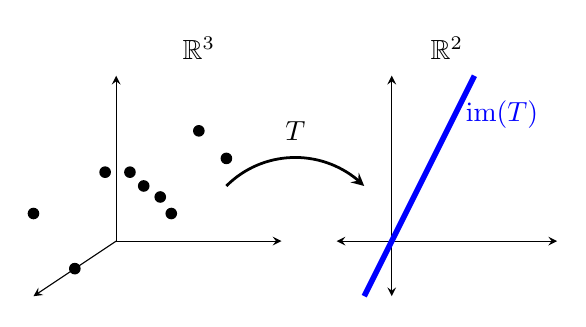
\begin{tikzpicture}[scale=.7]
     
      % Left image
      \node at (1.5, 3.5) {$\mathbb{R}^3$}; % Title for the left image
      \draw[->] (0,0)--(3,0); % x-axis
      \draw[->] (0,0)--(0,3); % y-axis
      \draw[->] (0,0)--(-1.5,-1); % diagonal axis
    
      % Random multicolored points in the left image
      \foreach \x/\y/\color in {0.5/1/red, 1/0.5/green, 1.5/2/blue, 2/1.5/orange, 0.8/0.8/purple, -1.5/.5/red, -.75/-.5/blue, -.2/1.25/red, .25/1.25/orange} {
        \fill[\color] (\x, \y) circle (3pt);
      }
      
      % Right image
      \node at (6, 3.5) {$\mathbb{R}^2$}; % Title for the right image
      \draw[<->] (4,0)--(8,0); % x-axis
      \draw[<->] (5,-1)--(5,3); % y-axis
      \draw[line width=2pt,blue] (4.5,-1)--(6.5,3); % diagonal line
    
      % Labels
      \node[] at (3.25, 2) (b) {$T$};
      \draw [->,line width=1pt,-stealth] (2,1) to[out=45] (4.5, 1);
      \node[blue] at (7, 2.3) (b) {$\mbox{im}(T)$};
     
    \end{tikzpicture}
\end{center}

Hence, the line $\mbox{span}\left(\begin{bmatrix}1\\2\end{bmatrix}\right)$ is a subspace of $\RR^2$, as is $\mbox{im}(T)$ and $\mbox{col}(A)$, where $T$ is the transformation associated with $A$.

\end{example}

\begin{example}

  Also recall that the null space of the matrix 

  $$B=\begin{bmatrix}
        1 & 3 & 2 & 0 & 0  \\
        0 & 1 & 5 & 2 & 1  \\
        3 & 5 & -14 & -8 &-4  \\
        0 & 0 & 0 & 1 & 1  \\
        \end{bmatrix}$$

  was the plane $Null(B)=\text{span}\left\{ \begin{bmatrix} 13 \\ -5 \\ 1 \\ 0 \\ 0 \end{bmatrix}, \begin{bmatrix} -3 \\ 1 \\ 0 \\ -1 \\ 1 \end{bmatrix} \right\}$.
  
  This planar null space is a subspace of $\RR^5$.

\end{example}

\begin{exploration}{Domain? Or Co-Domain?}

  One detail that is important, but often confuses students until they've had enough experience with these distinctions, is whether you're looking at the domain or co-domain of a function (aka transformation).

  The key is to remember whether you're thinking about \emph{input} vectors or \emph{output} vectors.

  In the case of $Null(B)=\text{span}\left\{ \begin{bmatrix} 13 \\ -5 \\ 1 \\ 0 \\ 0 \end{bmatrix}, \begin{bmatrix} -3 \\ 1 \\ 0 \\ -1 \\ 1 \end{bmatrix} \right\}$, we are looking at \emph{input vectors}, since the question of a null space is ``Which vectors \emph{get mapped} to $\vec{0}$?''

  In the case of transformation images, we're asking about the vectors that get \emph{mapped to}.

  So the line in the image

  \begin{center}
    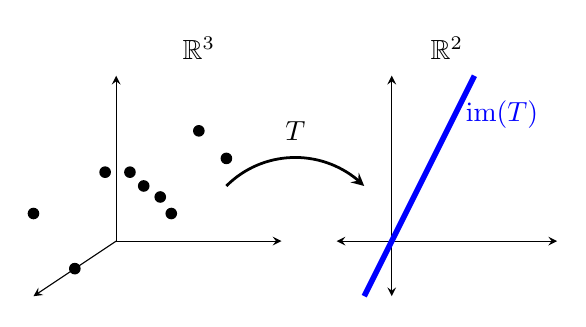
\begin{tikzpicture}[scale=.7]
     
      % Left image
      \node at (1.5, 3.5) {$\mathbb{R}^3$}; % Title for the left image
      \draw[->] (0,0)--(3,0); % x-axis
      \draw[->] (0,0)--(0,3); % y-axis
      \draw[->] (0,0)--(-1.5,-1); % diagonal axis
    
      % Random multicolored points in the left image
      \foreach \x/\y/\color in {0.5/1/red, 1/0.5/green, 1.5/2/blue, 2/1.5/orange, 0.8/0.8/purple, -1.5/.5/red, -.75/-.5/blue, -.2/1.25/red, .25/1.25/orange} {
        \fill[\color] (\x, \y) circle (3pt);
      }
      
      % Right image
      \node at (6, 3.5) {$\mathbb{R}^2$}; % Title for the right image
      \draw[<->] (4,0)--(8,0); % x-axis
      \draw[<->] (5,-1)--(5,3); % y-axis
      \draw[line width=2pt,blue] (4.5,-1)--(6.5,3); % diagonal line
    
      % Labels
      \node[] at (3.25, 2) (b) {$T$};
      \draw [->,line width=1pt,-stealth] (2,1) to[out=45] (4.5, 1);
      \node[blue] at (7, 2.3) (b) {$\mbox{im}(T)$};
     
    \end{tikzpicture}
\end{center}

is the set of \emph{output} vectors.

Hence, $\mbox{span}\left(\begin{bmatrix}1\\2\end{bmatrix}\right)$ is a subspace of the co-domain. 

\end{exploration}

\begin{remark}

  Images can be helpful for keeping ideas straight. 

  Here is an image depicting the fundamental spaces of matrices we've been discussing. To my knowledge, this was popularized by Gilbert Strang from MIT.

\begin{center}
  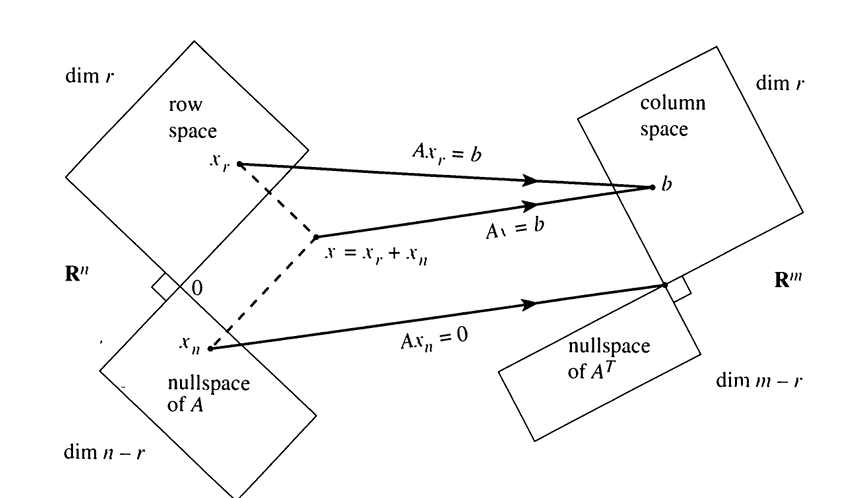
\includegraphics[width=22.46, height=13.18]{fundamental_spaces_1.png}
  %cite strang http://links.jstor.org/sici?sici=0002-9890%28199311%29100%3A9%3C848%3ATFTOLA%3E2.0.CO%3B2-A
\end{center}

\end{remark}

You might notice some extra terms, and also some claims about the dimensions of the spaces in this image.

We'll return to these in the next chapter. Fow now, we define the row space of a matrix and culminate in the Rank-Nullity Theorem.

We've been focusing on the \emph{column space} of a matrix $M$ because it gives us the image of the associated linear transformation. We can also talk about the \emph{row space}, which deals more with the domain of the transformation (in this case, the vectors that don't get mapped to $\vec{0}$)

\begin{definition}

  The \emph{row space} of a matrix $A$ is the span of its rows. 

\end{definition}

\begin{remark}

  You might notice in Strang's image that the vectors $x_r$ in the row space map to the column space of the matrix, and that the null space vectors $x_n$ map to $\vec{0}$. This is no coincidence, and the row space and null space only overlap at  $\vec{0}$. We'll unpack this more in the next chapter.

\end{remark}
 
You'll also notice that, according to Strang's image, $dim(\mbox{row}(A))+dim(\mbox{null}(A))=n$, and $dim(\mbox{col}(A))+dim(\mbox{null}(A^T))=m$. This is because of the Rank-Nullity Theorem.

\subsection*{Rank-Nullity Theorem for Linear Transformations}
 
\begin{definition}\label{def:nullityT}
The \dfn{nullity} of a linear transformation $T:V\rightarrow W$, is the dimension of the kernel of $T$.
$$\mbox{nullity}(T)=\mbox{dim}(\mbox{ker}(T))$$
\end{definition}

Earlier, we found the image and the kernel of the linear transformation $T:\RR^5\rightarrow \RR^4$ with standard matrix
 
$$A=\begin{bmatrix}1 & 2 & 2 &-1 & 0\\-1 & 3 & 1 & 0 & -1\\3 & 0 & 0 & 3 & 6\\ 1 & -1 & 1 & -2 & -1\end{bmatrix}$$
 
We also found that
$$\mbox{rank}(T)=\mbox{dim}(\mbox{im}(T))=\mbox{dim}(\mbox{col}(A))=\mbox{rank}(A)=3$$
and
$$\mbox{nullity}(T)=\mbox{dim}(\mbox{ker}(T))=\mbox{dim}(\mbox{null}(A))=\mbox{nullity}(A)=2$$
 
You might notice that
$$\mbox{rank}(T)+\mbox{nullity}(T)=3+2=5=\mbox{dim}(\RR^5),$$

the dimension of the domain space for $A$.
 
The following theorem confirms this property for all linear transformations.
 
\begin{theorem}\label{th:ranknullityforT}
Let $T:V\rightarrow W$ be a linear transformation, and its associated $m\times n$ matrix $A$. This means that $\mbox{dim}(V)=m$.

We can conclude that
$$\mbox{rank}(T)+\mbox{nullity}(T)=n$$
\end{theorem}
 
One consequence of this is that once you find the dimension of one of the related spaces (e.g. $\mbox{im}(A), \mbox{null}(A), \mbox{row}(A), \mbox{null}(A^T)$), you immediately know the dimensions of the other spaces!

Let's try it out.


Describe the properties of the matrix $A$ below, and the associated transformation $T$,

\begin{problem}\label{prob:imagerankoflintrans1}
$T:\RR^5\rightarrow \RR^2$, $A=\begin{bmatrix}3&2&4&7&1\\-1&-9&7&6&8\end{bmatrix}$.
  
\begin{selectAll}
\choice[correct]{$\mbox{im}(T)=\RR^2$}
\choice{$\mbox{im}(T)$ is a line in $\RR^2$}
\choice{$\mbox{null}(A)=\{\vec{0}\}$ }
\choice{$\mbox{im}(T)=\RR^5$}
\choice[correct]{$dim(\mbox{row}(A))=3$}
\choice{$\mbox{im}(T)$ is a plane in $\RR^5$}
\choice{$\mbox{rank}(A)=5$}
\choice[correct]{$\mbox{rank}(A)=2$}
\choice{$dim(\mbox{row}(A))=5$}
\choice{$\mbox{row}(A)=\RR^5$}
\choice[correct]{$\mbox{nullity}(A)=3$}
\choice[correct]{$dim(\mbox{null}(A^T))=3$}
\end{selectAll}
  
\begin{solution}

  If we take \texttt{rref(A)}, we get

  $$\begin{bmatrix}1&0&2&3&1\\0&1&-1&-1&-1\end{bmatrix}.$$

  At most, the image of $A$ would be $\RR^2$. Since the rank of $A$ is $2$ (note the two pivot columns), we indeed know that $\mbox{im}(A)=\RR^2$, as opposed to some line in $\RR^2$ (or $\vec{0}$.)

  This means that $\mbox{dim}(\mbox{ker}(T))=3$, so a $3$-dimensional subspace of $\RR^5$ maps to $\vec{0}$.

\end{solution}

Which vectors are in the kernel of $T$?

\begin{selectAll}

\choice{$\sigma\begin{bmatrix}7\\6\end{bmatrix}$}

\choice[correct]{$\tau\begin{bmatrix}-2\\1\\1\\0\\0\end{bmatrix}$}

\choice{$\tau\begin{bmatrix}-2\\1\\1\\0\\0\end{bmatrix}+\sigma\begin{bmatrix}0\\1\\0\\1\\0\end{bmatrix}+\rho\begin{bmatrix}-3\\1\\0\\1\\0\end{bmatrix}$}

\choice[correct]{$\tau\begin{bmatrix}-1\\1\\0\\0\\1\end{bmatrix}+\sigma\begin{bmatrix}-2\\1\\1\\0\\0\end{bmatrix}+\rho\begin{bmatrix}-3\\1\\0\\1\\0\end{bmatrix}$}

\choice{$\sigma\begin{bmatrix}3\\-1\end{bmatrix}+\sigma\begin{bmatrix}1\\8\end{bmatrix}+\sigma\begin{bmatrix}2\\-9\end{bmatrix}$}

\end{selectAll}

\end{problem}
 
 

\end{document}